\documentclass[11pt]{amsart}
\usepackage[margin=1.2in]{geometry}
\usepackage{amsmath,amssymb,amsthm}
\usepackage{xcolor}
\usepackage{tikz}
\usepackage[colorlinks=true,linkcolor=blue!60!black,citecolor=blue!60!black,urlcolor=blue!60!black,pdftitle={Flux rigidity for ancient single-mode solutions of the two-dimensional hydrostatic Euler equations},pdfauthor={Rifat Jumagulov},pdfsubject={Liouville-type flux rigidity on the single-mode strata of the two-dimensional hydrostatic Euler equations},pdfkeywords={hydrostatic Euler equations, ancient solutions, Liouville theorems, flux rigidity, level-set topology}]{hyperref}
\usepackage{microtype}

\newtheorem{theorem}{Theorem}[section]
\newtheorem{lemma}[theorem]{Lemma}
\newtheorem{proposition}[theorem]{Proposition}
\newtheorem{corollary}[theorem]{Corollary}
\theoremstyle{definition}
\newtheorem{definition}[theorem]{Definition}
\newtheorem{hypothesis}[theorem]{Hypothesis}
\theoremstyle{remark}
\newtheorem{remark}[theorem]{Remark}
\newtheorem{openproblem}[theorem]{Open problem}

\newcommand{\T}{\mathbb{T}}
\newcommand{\R}{\mathbb{R}}
\newcommand{\ZZmod}{\mathbb{Z}_2}
\newcommand{\Fbar}{\bar\Phi}
\newcommand{\mean}[1]{\langle #1\rangle}
\DeclareMathOperator{\intr}{int}
\DeclareMathOperator{\osc}{osc}

\title[Flux rigidity for ancient single-mode hydrostatic Euler flows]{Flux
rigidity for ancient single-mode solutions\\ of the two-dimensional
hydrostatic Euler equations}

\author{Rifat Jumagulov}
\email{jum.rifm@gmail.com}
%% Independent researcher; an institutional \address{...} is optional and may be added here.
\subjclass[2020]{35Q31, 35B53, 76B99}
\keywords{hydrostatic Euler equations, ancient solutions, Liouville
theorems, flux rigidity, level-set topology}
\date{July 2026}

\begin{document}

\begin{abstract}
We prove a Liouville-type flux-rigidity theorem for the two-dimensional
hydrostatic Euler equations on the periodic cell $\T^2$. For each $k\ge1$,
the class of exact solutions whose $\xi$-spectrum is supported on
$\{0,\pm k\}$ is exactly parametrized in Fourier form: an arbitrary smooth
mean profile $b(Z,\tau)$ transports an arbitrary initial fluctuation by
the accumulated shear, and the squared modal amplitude $S=P^2+Q^2$ is
time-independent. The main theorem states that every such solution which
is ancient, has uniformly bounded velocity component $v$ on
$\tau\le0$, and for which, at almost every time, no regular stream-function level
component is freely homotopic to a horizontal circle $\{Z=\mathrm{const}\}$, has
vanishing backward Ces\`aro mean flux
$\Fbar=-\overline{\mean{u^2v}}=0$. For a time-independent mean profile the
mechanism is secular; in general it combines an annular separation lemma
with an anchored estimate on the time-averaged shear. Each hypothesis is
necessary at every fixed $k$: explicit witnesses carry flux
$5k^2\varepsilon/8$ when the $v$-bound is dropped, and a
compensated-gap shear when a horizontal level is admitted. A cylinder analogue holds for time-independent mean
profiles; the multi-mode problem remains open.
\end{abstract}

\maketitle

\section{Introduction}\label{sec:intro}

The two-dimensional hydrostatic Euler equations (also called the
homogeneous hydrostatic equations) arise as the formal small-aspect-ratio
limit of the 2D incompressible Euler equations and as the inviscid
backbone of the Prandtl hierarchy. The rigorous theory around them is by
now substantial: see Grenier~\cite{Grenier1999} and
Brenier~\cite{Brenier1999} for the derivation of the limit and a
variational (optimal-transport) approach to well-posedness and
finite-time breakdown for convex profiles;
Masmoudi--Wong~\cite{MasmoudiWong2012} for the $H^s$ theory under
convexity, and Kukavica--Temam--Vicol--Ziane~\cite{KTVZ2011} and
Kukavica--Masmoudi--Vicol--Wong~\cite{KMVW2014} for local well-posedness
in analytic and structured classes; Renardy~\cite{Renardy2009} and
Han-Kwan--Nguyen~\cite{HKN2016} for ill-posedness outside such classes;
Wong~\cite{Wong2015} and Cao--Ibrahim--Nakanishi--Titi~\cite{CINT2015}
for finite-time blowup of smooth solutions; and
Boutros--Markfelder--Titi~\cite{BMT2024} for the modern weak-solution
theory, including nonuniqueness of generalised weak solutions. On the
periodic cell $\T^2\ni(\xi,Z)$ the system reads, for a stream function
$W(\xi,Z,\tau)$ with \emph{anisotropic vorticity} $w:=W_{\xi\xi}$,
\begin{equation}\label{eq:pde}
  w_\tau+\{W,w\}=0,\qquad \{A,B\}:=A_\xi B_Z-A_Z B_\xi,
\end{equation}
equivalently (see \S\ref{subsec:equiv})
\[
  u_\tau+v u_\xi+u u_Z=-p_Z,\qquad p_\xi=0,\qquad
  u=W_\xi,\quad v=-W_Z,\quad v_\xi+u_Z=0 .
\]
(Our variable names are adapted to the application below: $\xi$ is the
periodic ``fast'' direction carrying the wave, $Z$ the transverse
direction carrying the shear.)

Because the pressure is independent of $\xi$, the mean profile
$b:=\mean{W}_\xi$ has \emph{no prognostic equation}: averaging the
momentum equation in $\xi$ only pins the pressure gradient,
$p_Z=-\partial_Z\mean{u^2}_\xi$, and $b$ enters the dynamics of the
fluctuation only through the mean shear $V:=b_Z$. We call this the
\emph{undetermined mean sector}; it is the source of both the interest
and the difficulty of the problem studied here. (It is not a gauge
freedom: changing $b_Z$ changes the physical velocity $v=-W_Z$. The only
true gauge freedom of the stream function is $W\mapsto W+\beta_0(\tau)$,
which leaves $(u,v)$ unchanged; see \S\ref{subsec:frame}.)

The quantity of interest is the \emph{flux}
\begin{equation}\label{eq:flux}
  \Phi:=\mean{W_ZW_\xi^2}=-\mean{u^2v},
\end{equation}
where $\mean{\cdot}$ denotes the normalized average over $\T^2$
(\S\ref{subsec:conventions}), together with its \emph{ancient mean}
\begin{equation}\label{eq:fmean}
  \Fbar:=\lim_{T\to\infty}\frac1T\int_{-T}^0\Phi(\tau)\,d\tau
\end{equation}
(a backward Ces\`aro mean; on the classes treated below the limit is
shown to exist together with its value). With the horizontal kinetic
energy $e_h:=\tfrac12u^2$, the flux is
$\Phi=-\mean{u^2v}=-2\mean{v\,e_h}$: up to the conventional sign and the
factor~$2$, it is the spatially averaged transverse advective transport of
horizontal kinetic energy by the velocity component $v$ --- a third-order
velocity correlation, not the flux of a conserved density
(Remark~\ref{rem:observable}), and the natural scalar diagnostic of the
undetermined mean sector against the wave. The unnormalized form
$-\mean{u^2v}$ (without the factor $\tfrac12$) is chosen for the cleaner
identity $\Phi=\tfrac{k^2}{4\pi}\oint b_ZS\,dZ$ below. Its status as an
observable, the normalization of the velocity field, and its behavior
under Galilean boosts are discussed in
Remarks~\ref{rem:frame} and~\ref{rem:observable}.

We work in the genre of Liouville theorems for \emph{ancient bounded}
solutions, in the spirit of Koch--Nadirashvili--Seregin--\v Sver\'ak
\cite{KNSS2009} for the Navier--Stokes equations, of the Liouville
theorem of Hamel--Nadirashvili \cite{HamelNadirashvili2019} for the
two-dimensional Euler equations, and of the axisymmetric
rigidity theorem of Lei--Zhang \cite{LeiZhang2011}: one restricts
attention to solutions defined on the whole backward time axis
$\tau\in(-\infty,0]$ and satisfying uniform bounds, and asks which
transport can survive. Two hypotheses are used; they are exactly those consumed by the proofs
below, and each is shown --- at every fixed harmonic --- to be
individually non-removable in Section~\ref{sec:sharpness}. (We do not
claim minimality against every conceivable weakening: for instance the
uniform bound on $v$ could in principle be relaxed to a direct control
of the accumulated phase; the point is that neither hypothesis can be
dropped outright.)

\begin{hypothesis}[Ancient $v$-bound]\label{hyp:v}
$W$ is a solution of \eqref{eq:pde} on $\tau\in(-\infty,0]$ with
\[
  C_v:=\sup_{\tau\le0}\|v(\cdot,\cdot,\tau)\|_{L^\infty}<\infty .
\]
\end{hypothesis}

\begin{hypothesis}[No horizontal level]\label{hyp:conf}
For a.e.\ $\tau\le0$ (with respect to Lebesgue measure) and every regular
value $c$ of $W(\cdot,\cdot,\tau)$ --- that is, every $c$ outside the
null set of critical values furnished by Sard's theorem --- no connected
component of the level set $\{W(\cdot,\cdot,\tau)=c\}$ is freely homotopic
in $\T^2$ to a horizontal circle $\{Z=\mathrm{const}\}$; equivalently,
after choosing an orientation, no such component represents
$\pm(1,0)\in H_1(\T^2;\mathbb Z)$.
\end{hypothesis}

Hypothesis~\ref{hyp:conf} forbids exactly one topological event: a
regular level component that wraps the torus horizontally, in the sense
of being freely homotopic to a circle $\{Z=\mathrm{const}\}$ --- integer
class $\pm(1,0)$, i.e.\ winding once in $\xi$ and \emph{zero} times in
$Z$. Every other class is allowed: vertical winding, and diagonal classes
such as the $(1,1)$-levels of $\cos(\xi-Z)$
(Remark~\ref{rem:sharpness-k}); so is arbitrary behavior at critical
values. Only the free-homotopy class --- not its mod-$2$ reduction --- is
used: the separating level produced in the annular argument
(Lemma~\ref{lem:annulus-top}) is an \emph{embedded essential} circle,
hence isotopic to the core of its annulus and of integer class exactly
$\pm(1,0)$, so classes such as $(1,2)$ (which a mod-$2$ condition would
also forbid) never arise and are left admissible. The conventions are
discussed in Remark~\ref{rem:conventions}.

\subsection*{Main results}

The object of this paper is the \emph{single-mode stratum of harmonic
$k$}: solutions whose $\xi$-spectrum lies in $\{0,\pm k\}$, for a fixed
integer $k\ge1$. Our first result (Lemma~\ref{lem:class-cartesian}) is
that each such class is closed under the evolution and admits an exact
parametrization in Fourier form:
\[
  W \;=\; b(Z,\tau)
  +P_0(Z)\cos\bigl(k\xi+k\,\partial_ZB(Z,\tau)\bigr)
  +Q_0(Z)\sin\bigl(k\xi+k\,\partial_ZB(Z,\tau)\bigr),
\]
with $B(Z,\tau):=\int_0^\tau b(Z,s)\,ds$: the fluctuation at time $\tau$
is the initial fluctuation composed with the accumulated shear,
$W'(\xi,Z,\tau)=W'_0(\xi+\partial_ZB(Z,\tau),Z)$, uniformly in $k$. In
particular the \emph{squared modal amplitude} $S:=P^2+Q^2=P_0^2+Q_0^2$ is
time-independent, while the mean profile $b$ remains completely free (the
undetermined mean sector). On this class the flux is a pure mean-shear
channel:
\[
  \Phi(\tau)=\frac{k^2}{4\pi}\oint b_Z(Z,\tau)\,S(Z)\,dZ .
\]

\begin{theorem}[Flux rigidity on the single-mode strata]
\label{thm:main-intro}
Fix $k\ge1$ and let $W$ be a single-mode solution of harmonic $k$
--- smooth on $\T^2\times(-\infty,0]$, with $\xi$-spectrum in
$\{0,\pm k\}$ --- satisfying Hypotheses~\ref{hyp:v} and~\ref{hyp:conf}.
Then the ancient mean flux exists and vanishes: $\Fbar=0$.
\end{theorem}

\begin{corollary}[KNSS-type form]\label{cor:knss}
The conclusion holds, in particular, for every single-mode solution which
is ancient with \emph{both} velocity components uniformly bounded and
\emph{confined}, i.e.\ such that for a.e.\ $\tau$ every regular level
component of $W(\cdot,\cdot,\tau)$ is contractible in $\T^2$.
\end{corollary}

Indeed, a contractible component is null-homotopic, hence not freely
homotopic to any essential circle --- in particular not to a horizontal
one --- so confinement implies Hypothesis~\ref{hyp:conf}; and
boundedness of both components implies Hypothesis~\ref{hyp:v}. We
emphasize that the corollary's hypotheses are strictly stronger than the
theorem's: on the single-mode class the $u$-bound is automatic
($\sup_\xi|u|=k\sqrt S$ is finite and time-independent by
Lemma~\ref{lem:class-cartesian}), and full contractibility excludes even
the standing wave $W=\sin(k\xi)$, whose regular levels are vertical
circles, while Hypothesis~\ref{hyp:conf} admits it. The witnesses of
Section~\ref{sec:sharpness} show that Hypotheses~\ref{hyp:v}
and~\ref{hyp:conf} are each individually necessary, at every fixed
harmonic (Remark~\ref{rem:sharpness-k}).

The proof splits into two regimes: the separation topology that enforces
Hypothesis~\ref{hyp:conf} is common to both (Remark~\ref{rem:unified}),
but the analytic obstruction differs. (The one-line assembly of
Theorem~\ref{thm:main-intro} is given at the end of
Section~\ref{sec:full}.)

\emph{Time-independent mean profile} ($b=b(Z)$; Theorem~\ref{thm:static}).
Here the evolution is a shear conjugacy, level topology is frozen in
time, and the mechanism is \emph{secular}: the velocity component $v$
contains a term of amplitude $k\,\sqrt{S(Z)}\,|b''(Z)|\,|\tau|$, so any
$Z$ with $S(Z)b''(Z)\neq0$ makes $\sup|v|$ grow linearly in backward time
--- \textbf{flux costs unbounded~$v$}. The velocity bound therefore
forces $b''\equiv0$ on $\{S>0\}$, Hypothesis~\ref{hyp:conf} forces
$b'\equiv0$ on the interior of $\{S=0\}$ (a horizontal circle in a
spectral gap is itself such a level), and a
density-plus-continuity argument propagates $b''\equiv0$ to all of $\T$,
whence $b'\equiv c_0$ and finally $c_0=0$.

\emph{Time-dependent mean profile} (Theorem~\ref{thm:full}). Here the
conjugacy structure is lost and level topology is \emph{not} frozen. A
serious candidate configuration exists at the formal level:
backward-sharpening averaged-shear fronts located at simple zeros of
$\sqrt S$, which satisfy the $v$-bound by exact saturation and arrange
their zero circles to be critical --- mean shear dominated by $|X_0'|$
there --- hence exempt from Hypothesis~\ref{hyp:conf} (a front whose
zero circles were instead regular would violate the hypothesis
outright). The theorem is nevertheless true, by a different mechanism
which we isolate as an \emph{annular separation} argument
(Lemmas~\ref{lem:annulus-top} and~\ref{lem:annular}): on the closed
annulus between two consecutive zeros of $\sqrt S$ the stream function
is constant on each boundary circle; if the two boundary values differ,
every intermediate Sard-regular level separates the ends of the annulus,
and a finite union of components none of which is freely homotopic to the
core cannot separate --- so some component is freely homotopic to a
horizontal circle, violating Hypothesis~\ref{hyp:conf}. This pins the mean profile,
$b(z_{j+1},\tau)=b(z_j,\tau)$ for every $\tau$, on every arc between
consecutive zeros of $\sqrt S$. An anchored estimate derived from the
$v$-bound, $k\sqrt S\,|\partial_Z\bar V_T|\le K_0/T$ with
$K_0=2C_v+\|(P_0',Q_0')\|_\infty$, for the backward time-average
$\bar V_T$ of the shear, then forces the averaged shear to
equidistribute to zero against the weight $S$, and $\Fbar=0$ follows.

The two hypotheses are each necessary, at every fixed harmonic
(Section~\ref{sec:sharpness}):
dropping the $v$-bound admits the explicit flux-carrying witness of
Proposition~\ref{prop:counterexample}, and admitting a horizontal level
admits a compensated-gap shear witness
(Proposition~\ref{prop:gapwitness}). The theorem for time-independent
mean profiles has a cylinder analogue (Theorem~\ref{thm:cylinder}); the
optimal cylinder statement for time-dependent mean profiles is left open
(Remark~\ref{rem:cylinder-full}).

\subsection*{Context and scope}

Steady cells ($b_Z\equiv0$) are the classical zero-flux members of the
ancient class. (Traveling waves in $\xi$ obtained by a Galilean boost lie
outside the periodic-stream-function rest frame used here --- the boost
adds $-cZ$, breaking $Z$-periodicity, and shifts the flux by
$\Phi\mapsto\Phi-c\mean{u^2}$, Remark~\ref{rem:frame}. A rigid
$\xi$-translation of the wave \emph{within} the periodic class forces
$b_Z$ to be constant on $\{S>0\}$: a globally constant $b_Z\equiv-c$ is
the non-periodic $b=-cZ$, whereas the periodic alternative --- $b_Z$
constant on the wave support, compensated in a spectral gap --- does
exist, but is exactly the flux-carrying compensated-gap witness of
Proposition~\ref{prop:gapwitness}, which violates
Hypothesis~\ref{hyp:conf}. Either way it is not a zero-flux member of the
confined class.) For \emph{steady} hydrostatic
flows rigidity results are available: Leung--Wong--Xie \cite{LWX2024}
prove, as one ingredient of their characterization of steady nozzle
flows, that steady solutions in an infinite strip strictly away from
stagnation are shear flows (see also the references there). Rigidity of a
different flavour appears for neighbouring geophysical systems:
Peralta-Salas--Slobodeanu \cite{PeraltaSlobodeanu2023} prove the
nonexistence of smooth compactly supported \emph{stationary} solutions of
the $3$D primitive equations, and Martin \cite{Martin2023} obtains
Liouville-type results for time-dependent stratified flows in the
$\beta$-plane. On the conserved-quantity side, in the spirit of Onsager's conjecture
for the hydrostatic Euler equations, sufficient regularity criteria for
conservation of the horizontal kinetic energy of weak solutions are
established by Boutros--Markfelder--Titi \cite{BMTOnsager2023}.

The present result concerns the genuinely time-dependent ancient regime,
where the freedom of the undetermined mean sector is the central
difficulty. Its novelty is not the single-mode classification (which
follows by substitution) but the combination of three ingredients: the
exact phase-evolution formula \eqref{eq:full-class}, the representation of
the flux as the weighted mean shear
$\Phi=\tfrac{k^2}{4\pi}\oint b_Z S\,dZ$, and the topological argument by
which the transverse-velocity bound and the no-horizontal-level
hypothesis together force $\Fbar=0$. With the classification stated in
Fourier form, the theorem covers each single-mode stratum in full. The
multi-mode problem remains open --- to the best of the author's
knowledge, no Liouville-type result is available for the time-dependent
ancient regime of the hydrostatic Euler equations beyond the single-mode
strata --- and appears to be of a different nature; we state it precisely
in Section~\ref{sec:open}. We do not claim any consequence at the level
of the primitive (axisymmetric Navier--Stokes) equations.

A remark on verification: the classification identities of
Lemma~\ref{lem:class-cartesian}, the flux formula, and the
counterexample's flux value are verified in exact (symbolic) arithmetic,
and the counterexample's residual and secular growth in float64 grid
arithmetic, by short standalone scripts that accompany this paper as
ancillary files (Appendix~\ref{app:verification}); none is load-bearing
for the proofs, which are complete in the text. A plausible-but-false
variant of one step, worth flagging for arguments of this genre, is
discussed in Remark~\ref{rem:adjacency}.

\section{Setting}\label{sec:setting}

Throughout, $\T=\R/2\pi\mathbb{Z}$ and $\T^2\ni(\xi,Z)$; all functions
are smooth unless stated otherwise (for the time-independent mean
profile, $C^2$ regularity suffices; see Remark~\ref{rem:regularity}).

\subsection{Conventions}\label{subsec:conventions}
Averages are normalized:
\[
  \mean{f}:=\frac1{4\pi^2}\int_0^{2\pi}\!\!\int_0^{2\pi}
  f(\xi,Z)\,d\xi\,dZ,
  \qquad
  \mean{f}_\xi:=\frac1{2\pi}\int_0^{2\pi}f(\xi,Z)\,d\xi ,
\]
and $\oint$ denotes $\int_0^{2\pi}\cdot\,dZ$. The system is
\eqref{eq:pde} with $u=W_\xi$, $v=-W_Z$, $w=W_{\xi\xi}=u_\xi$. The flux
is \eqref{eq:flux}; note that $\mean{W_ZW_\xi^2}=-\mean{u^2v}$ holds
pointwise, since $v=-W_Z$ (both forms will be used).

\subsection{Equivalence with the momentum form; pressure recovery}
\label{subsec:equiv}
Given a solution of the momentum form, differentiating
$u_\tau+vu_\xi+uu_Z=-p_Z$ in $\xi$ eliminates the pressure and, using
$v_\xi+u_Z=0$, yields \eqref{eq:pde} for $w=u_\xi$. Conversely, given a
solution $W$ of \eqref{eq:pde}, average the momentum equation in $\xi$:
since $\mean{u}_\xi\equiv0$ and
$\mean{vu_\xi+uu_Z}_\xi=\partial_Z\mean{u^2}_\xi$ (integrate the first
term by parts in $\xi$ and use $v_\xi=-u_Z$), the pressure is recovered,
up to a function of time, by
\[
  p_Z=-\partial_Z\mean{u^2}_\xi ,
\]
and the fluctuating part of the momentum equation is the
$\partial_\xi$-antiderivative of \eqref{eq:pde}. This justifies
``equivalently'' above.

\subsection{The undetermined mean sector; frame normalization}
\label{subsec:frame}
Decomposing $W=b(Z,\tau)+W'$ with $\mean{W'}_\xi=0$: there is no
evolution equation for $b$; the mean profile is a free trajectory of the
undetermined mean sector, constrained only through its interaction with
the fluctuation, which happens exclusively through the mean shear
$V=b_Z$. The true gauge freedom is $W\mapsto W+\beta_0(\tau)$, which
leaves $(u,v)$ --- and hence $\Phi$ and $\Fbar$ --- unchanged.

\begin{remark}[Circulations and Galilean frame]\label{rem:frame}
The velocity field of \eqref{eq:pde} is $(\dot\xi,\dot Z)=(v,u)$. On
$\T^2$ a general divergence-free field carries two harmonic (constant)
components; the representation by a \emph{periodic} stream function
fixes them to zero: $\mean{u}=\mean{W_\xi}=0$ and
$\mean{v}=-\mean{W_Z}=0$. The setting thus selects the canonical rest
frame of zero mean velocity. A Galilean boost along $\xi$ acts by
$\widetilde W(\xi,Z,\tau)=W(\xi-c\tau,Z,\tau)-cZ$, so that
$\widetilde v=v(\xi-c\tau,\cdot,\cdot)+c$ and
$\widetilde u=u(\xi-c\tau,\cdot,\cdot)$ and the equation is preserved;
the boosted stream function is no longer $Z$-periodic, and the flux
shifts by
\[
  \Phi\;\longmapsto\;\Phi-c\,\mean{u^2},
\]
with $\mean{u^2}=\tfrac{k^2}{4\pi}\oint S\,dZ$ conserved on the classes
below; the value of $\Phi$ is therefore frame-dependent, and
Theorem~\ref{thm:main-intro} is a statement in the canonical rest frame.
Because the boost adds the term $-cZ$ it breaks $Z$-periodicity, so no
nontrivial $\xi$-boost preserves the periodic class; the level-set
hypothesis (Hypothesis~\ref{hyp:conf}), like $\Phi$ itself, is thus
intrinsically a rest-frame condition.
\end{remark}

\begin{remark}[The flux as an observable]\label{rem:observable}
The flux \eqref{eq:flux} is not the transport of a conserved density:
the $\xi$-averaged budget of the (hydrostatic) kinetic energy reads, for
every solution,
\[
  \partial_\tau\mean{\tfrac12u^2}_\xi
  +\partial_Z\mean{\tfrac12u^3}_\xi=0
\]
(multiply the momentum equation by $u$, average in $\xi$, and use
$p_\xi=0$, $\mean{u}_\xi=0$, $v_\xi=-u_Z$), and on the single-mode class
both terms vanish separately ($\mean{u^2}_\xi=\tfrac{k^2}2S$ is
time-independent and $\mean{u^3}_\xi\equiv0$ by parity). Rather, on the
class the flux reduces to the pairing $\Phi=\mean{V\,\mean{u^2}_\xi}$ of
the \emph{undetermined} mean shear with the conserved modal weight
(Lemma~\ref{lem:flux}): it is the natural scalar diagnostic of the mean
sector against the wave, and since $b$ obeys no equation, a constraint
on $\Fbar$ is genuinely a constraint on which mean trajectories the
class admits, not a consequence of a closed balance law. The theorem
shows that, for ancient solutions satisfying
Hypotheses~\ref{hyp:v} and~\ref{hyp:conf}, no persistent correlation
between the mean shear and the modal weight can survive in the Ces\`aro
mean.
\end{remark}

\begin{remark}[Conventions in Hypothesis~\ref{hyp:conf}]
\label{rem:conventions}
(i) The quantifier is over \emph{components}: a level set may have
several components, and the hypothesis constrains each one separately
(replacing ``component'' by ``union of components'' would give a
different, and for our purposes wrong, condition). (ii) The hypothesis
is stated per regular \emph{value}; this single reading is used at both
consumption sites (Step~3 of Theorem~\ref{thm:static},
Lemma~\ref{lem:annular}). Under the alternative per-\emph{component}
reading --- forbidding a horizontal level for every component on which
$\nabla W\neq0$, regardless of the value --- the theorems also hold,
with slightly lower regularity requirements
(Remark~\ref{rem:regularity}). (iii) The condition is stated by free
homotopy (integer class $\pm(1,0)$), not by its mod-$2$ reduction. This
is exactly what the proofs use --- the only components they ever produce
are embedded essential annular circles, of integer class exactly
$\pm(1,0)$ (Lemma~\ref{lem:annulus-top}) --- so a mod-$2$ formulation
would forbid strictly more (e.g.\ class $(1,2)$) with no gain. A
by-product is \emph{cover-invariance}: the condition is preserved under
the $k$-fold covers $\eta_k(\xi,Z)=(k\xi,Z)$ of
Section~\ref{sec:sharpness} (a component is horizontal iff its
$\eta_k$-image is), which the mod-$2$ condition is not.
\end{remark}

\section{The single-mode classes}\label{sec:class}

Fix an integer $k\ge1$.

\begin{lemma}[Classification; Fourier form]\label{lem:class-cartesian}
Let $W$ be smooth on $\T^2\times(-\infty,0]$ with $\xi$-spectrum in
$\{0,\pm k\}$ for every $\tau$, and write
\[
  W=b(Z,\tau)+P(Z,\tau)\cos(k\xi)+Q(Z,\tau)\sin(k\xi) .
\]
Then $W$ solves \eqref{eq:pde} if and only if
\begin{equation}\label{eq:rotationlaw}
  \partial_\tau(P,Q)=k\,b_Z\,(Q,-P),
\end{equation}
with the mean profile $b$ unconstrained (the undetermined mean sector of
\S\ref{subsec:frame}). Equivalently, with
$B(Z,\tau):=\int_0^\tau b(Z,s)\,ds$ and $(P_0,Q_0):=(P,Q)(\cdot,0)$,
\begin{equation}\label{eq:full-class}
  W=b(Z,\tau)+P_0(Z)\cos\bigl(k\xi+k\,\partial_ZB(Z,\tau)\bigr)
   +Q_0(Z)\sin\bigl(k\xi+k\,\partial_ZB(Z,\tau)\bigr):
\end{equation}
the fluctuation at time $\tau$ is the initial fluctuation composed with
the accumulated shear,
$W'(\xi,Z,\tau)=W'_0\bigl(\xi+\partial_ZB(Z,\tau),Z\bigr)$, uniformly in
$k$. In particular the \emph{squared modal amplitude}
\[
  S(Z):=P^2+Q^2=P_0^2+Q_0^2
\]
(so that $\sqrt S$ is the wave amplitude and, by Lemma~\ref{lem:flux},
$\mean{u^2}_\xi=\tfrac{k^2}2S$ is the mean square of the wave velocity,
whose horizontal kinetic energy is $\mean{\tfrac12u^2}_\xi=\tfrac{k^2}4S$)
is time-independent, and \eqref{eq:full-class} is \emph{exactly} the
single-mode class of harmonic $k$: every such solution is realized by
exactly one pair of smooth $2\pi$-periodic Fourier coefficients
$(P_0,Q_0)$ and one smooth mean trajectory $b(\cdot,\cdot)$, namely its
own.
\end{lemma}

\begin{proof}
With $W'=P\cos(k\xi)+Q\sin(k\xi)$ one has $w=W_{\xi\xi}=-k^2W'$, so
$\{W',w\}=-k^2\{W',W'\}=0$ identically: the fluctuation self-interaction
of a single harmonic is null (no $m=\pm2k$ modes are generated, and the
class is closed under the evolution). Hence
\[
  \{W,w\}=\{b,w\}=-b_Z\,\partial_\xi w
  =k^3\,b_Z\,\bigl(Q\cos(k\xi)-P\sin(k\xi)\bigr),
\]
while $w_\tau=-k^2\bigl(P_\tau\cos(k\xi)+Q_\tau\sin(k\xi)\bigr)$;
matching the $\cos(k\xi)$ and $\sin(k\xi)$ coefficients of
$w_\tau+\{W,w\}=0$ gives exactly \eqref{eq:rotationlaw}, and the $m=0$
sector of the vorticity equation is empty, leaving $b$ free. Writing
$\zeta:=P+iQ$, \eqref{eq:rotationlaw} reads
$\zeta_\tau=-ik\,b_Z\,\zeta$, whence
$\zeta(Z,\tau)=e^{-ik\,\partial_ZB(Z,\tau)}\,\zeta_0(Z)$ (note
$\partial_ZB=\int_0^\tau b_Z$), which is \eqref{eq:full-class}; in
particular $S=|\zeta|^2$ is conserved. Conversely,
\eqref{eq:full-class} defines an exact solution for every smooth datum
by the same computation. Uniqueness of the realization is immediate:
$b=\mean{W}_\xi$ and $(P_0,Q_0)$ are the Fourier coefficients of
$W(\cdot,\cdot,0)$. The identities of this proof are additionally
machine-verified in exact symbolic arithmetic
(Appendix~\ref{app:verification}).
\end{proof}

\begin{lemma}[Time-independent mean profile; shear conjugacy]
\label{lem:class-static}
If $b=b(Z)$ is time-independent, \eqref{eq:full-class} becomes
\begin{equation}\label{eq:static-class}
  W=b(Z)+P_0(Z)\cos\bigl(k\xi+k\,b'(Z)\,\tau\bigr)
   +Q_0(Z)\sin\bigl(k\xi+k\,b'(Z)\,\tau\bigr)
  \;=\;W_0\circ H_\tau,
\end{equation}
where $H_\tau(\xi,Z)=(\xi+b'(Z)\tau,\,Z)$: the evolution is a shear
conjugacy by a diffeomorphism of $\T^2$ isotopic to the identity; in
particular the component topology of every level set is frozen in time.
\end{lemma}

\begin{proof}
Immediate from \eqref{eq:full-class} with
$\partial_ZB(Z,\tau)=b'(Z)\tau$.
\end{proof}

\begin{remark}[Polar form; two obstructions to a global amplitude--phase
pair]\label{rem:polar}
Where a smooth $2\pi$-periodic pair $(A,\varphi_0)$ with
$W'_0=A(Z)\sin\bigl(k\xi+k\varphi_0(Z)\bigr)$ exists,
\eqref{eq:full-class} takes the amplitude--phase form
\begin{equation}\label{eq:polar-form}
  W=b(Z,\tau)
  +A(Z)\,\sin\bigl(k\xi+k\varphi_0(Z)+k\,\partial_ZB(Z,\tau)\bigr),
  \qquad A^2=S ,
\end{equation}
which we use below to write down explicit witnesses
(Proposition~\ref{prop:counterexample}, Remark~\ref{rem:consistency},
Proposition~\ref{prop:gapwitness}). But not every single-mode field
admits such a pair, for two distinct reasons, so \eqref{eq:polar-form}
parametrizes a \emph{proper} subclass of the stratum.
(i) \emph{Phase winding}: for $W=\cos(\xi-Z)$ --- a smooth steady $k=1$
solution with spectrum $\{\pm1\}$ --- any polar phase equals $\pi/2-Z$
modulo $2\pi$ and sign, which has winding $-1$ in $Z$ and admits no
$2\pi$-periodic real-valued choice; and since $\varphi_0+\partial_ZB$ is
a sum of $2\pi$-periodic functions, the form \eqref{eq:polar-form} can
never produce a winding phase.
(ii) \emph{Sign lifting through zeros}: for
$(P_0,Q_0)=\cos(Z/2)\,\bigl(\cos(Z/2),\sin(Z/2)\bigr)$ (a $k=1$ datum),
smooth and $2\pi$-periodic with $S=(1+\cos Z)/2$, any smooth signed
amplitude equals $\pm\cos(Z/2)$ near the simple zero at $Z=\pi$, and
$C^1$-matching there forces one global sign, which is incompatible with
periodicity ($A(0)=-A(2\pi)$); only an \emph{antiperiodic} pair
represents this field. For these reasons the classification above, the
flux formula, and every estimate in
Sections~\ref{sec:static}--\ref{sec:cylinder} are stated and proved in
the representation-free variables $(P_0,Q_0)$, $S$, $\partial_ZB$ only.
\end{remark}

\begin{lemma}[Flux formula]\label{lem:flux}
On the class \eqref{eq:full-class},
\begin{equation}\label{eq:fluxformula}
  \mean{W_Zu^2}_\xi=\tfrac{k^2}2\,b_Z(Z,\tau)\,S(Z)
  \qquad\Longrightarrow\qquad
  \Phi(\tau)=\frac{k^2}{4\pi}\oint b_Z(Z,\tau)\,S(Z)\,dZ .
\end{equation}
In the decomposition of the flux into mean-shear and fluctuation
channels, $\Phi=\mean{V\,\mean{u^2}_\xi}+\mean{W'_Zu^2}$ with $W'$ the
$\xi$-fluctuation of $W$, the fluctuation channel vanishes identically
on the class by $\xi$-parity: the single-mode flux is a pure mean-shear
channel. For a time-independent mean profile \eqref{eq:static-class},
$\Phi$ is time-independent and $\Fbar=\frac{k^2}{4\pi}\oint b'S\,dZ$.
\end{lemma}

\begin{proof}
$u=W'_\xi=k\bigl(-P\sin(k\xi)+Q\cos(k\xi)\bigr)$, so
$\mean{u^2}_\xi=\tfrac{k^2}2(P^2+Q^2)=\tfrac{k^2}2S$ and
$\mean{W_Zu^2}_\xi=b_Z\mean{u^2}_\xi+\mean{W'_Zu^2}_\xi$. In the second
term, $W'_Z=P_Z\cos(k\xi)+Q_Z\sin(k\xi)$ multiplies
$u^2=k^2\bigl(P^2\sin^2-2PQ\sin\cos+Q^2\cos^2\bigr)(k\xi)$, producing
only odd trigonometric moments
($\mean{\cos^3}=\mean{\sin^3}=\mean{\sin\cos^2}=\mean{\sin^2\cos}=0$
over a period), so it vanishes; the first term is $\tfrac{k^2}2b_ZS$,
which gives \eqref{eq:fluxformula} after averaging over $Z$ ($S$ is
time-independent by Lemma~\ref{lem:class-cartesian}).
\end{proof}

\section{The time-independent mean profile}\label{sec:static}

\begin{theorem}[Single-mode strata, time-independent mean profile;
``flux costs unbounded $v$'']\label{thm:static}
Let $W$ be a single-mode solution \eqref{eq:static-class} with
time-independent mean profile, satisfying
Hypotheses~\ref{hyp:v} and~\ref{hyp:conf}. Then $b'\equiv0$ on $\T$:
the mean profile is constant. In particular $b'S\equiv0$ and $\Fbar=0$.
\end{theorem}

\begin{proof}
\emph{Step 1 (the secular term).} Write $X_0:=(P_0,Q_0)$,
$JX_0:=(Q_0,-P_0)$, and $\zeta_0:=P_0+iQ_0$. From
\eqref{eq:static-class},
\begin{equation}\label{eq:v-static}
\begin{aligned}
  v&=-W_Z=-\,b'(Z)-\bigl(P_Z\cos(k\xi)+Q_Z\sin(k\xi)\bigr),\\
  \sup_\xi\bigl|P_Z\cos(k\xi)+Q_Z\sin(k\xi)\bigr|
  &=\bigl|X_0'(Z)+k\,\tau\,b''(Z)\,JX_0(Z)\bigr|,
\end{aligned}
\end{equation}
where the identity on the second line holds because
$\zeta:=P+iQ=e^{-ik b'(Z)\tau}\zeta_0$
(Lemma~\ref{lem:class-cartesian}) gives
$\zeta_Z=e^{-ik b'\tau}\bigl(\zeta_0'-ik\tau b''\zeta_0\bigr)$, the
modulus is rotation-invariant, and $\zeta_0'-ik\tau b''\zeta_0$ is the
complex form of $X_0'+k\tau b''JX_0$. Every contribution to $v$ is
bounded uniformly in $\tau$ except the secular one: since
$|JX_0|=\sqrt S$,
\[
  \sup_{\T^2}\,|v(\cdot,\cdot,\tau)|
  \;\ge\;k\,|\tau|\,|b''(Z)|\sqrt{S(Z)}-|X_0'(Z)|-|b'(Z)|
  \qquad\text{for every }Z .
\]
If $S(Z)b''(Z)\neq0$ for some $Z$, the right side tends to $\infty$ as
$\tau\to-\infty$, contradicting Hypothesis~\ref{hyp:v}. Hence
\[
  S(Z)\,b''(Z)\equiv0\quad\text{on }\T .
\]

\emph{Step 2 (structure of $b'$ on the wave support).} Let
$\Omega:=\{Z:S(Z)>0\}$, an open subset of the circle. By Step~1,
$b''\equiv0$ on $\Omega$, so $b'$ is constant on each connected
component of $\Omega$.

\emph{Step 3 (spectral gaps).} Let $I\subseteq\intr\{S=0\}$ be a
nonempty open interval (a \emph{gap}; $\intr$ denotes the interior of a
set). On $\T_\xi\times I$ the solution is $W=b(Z)$: no
$\xi$-dependence. Suppose $b'(Z_0)\neq0$ for some $Z_0\in I$.
Pick a closed subinterval $J\subset I$ with $b'\neq0$ on $J$; then
$b(J)$ is a nondegenerate interval, and by Sard's theorem a.e.\
$c^*\in b(J)$ is a regular value of $W(\cdot,\cdot,\tau)$. For any such
$c^*=b(Z^*)$, $Z^*\in J$, the connected component of
$\{W(\cdot,\cdot,\tau)=c^*\}$ through $(\cdot,Z^*)$ is exactly the
horizontal circle $\{Z=Z^*\}$. Indeed, on $\T_\xi\times I$ one has
$W=b(Z)$; since $b'(Z^*)\neq0$, $b$ is strictly monotone on a collar
$U\ni Z^*$ in which $b(Z)=c^*$ holds only at $Z=Z^*$, so $\{Z=Z^*\}$ is
open in the level set $\{W=c^*\}$; being also compact, it is closed in
that level (which is regular, $|\nabla W|=|b'(Z^*)|\neq0$), hence a full
connected component --- freely homotopic to a horizontal circle. The gap region is invariant under the
shear conjugacy of Lemma~\ref{lem:class-static}, so this component
persists for all $\tau$, violating Hypothesis~\ref{hyp:conf}. Hence
$b'\equiv0$ on $\intr\{S=0\}$ (and so also $b''\equiv0$ there).

\emph{Step 4 (density).} By Steps 2 and 3, $b''=0$ on the open set
$\Omega\cup\intr\{S=0\}$, which is \emph{dense} in $\T$: its complement
is $\{S=0\}\setminus\intr\{S=0\}$, every point of which is a limit of
points of $\Omega$. Since $b''$ is continuous, $b''\equiv0$ on $\T$, so
$b'\equiv c_0$ is a global constant. If a gap exists, $c_0=0$ directly
by Step~3; if $\{S=0\}$ has empty interior, periodicity gives
$\oint b'\,dZ=0$, hence again $c_0=0$, i.e.\ $b'\equiv0$. In
particular $b'S\equiv0$ and, by Lemma~\ref{lem:flux},
$\Fbar=\frac{k^2}{4\pi}\oint b'S\,dZ=0$.
\end{proof}

\begin{remark}[Mechanism]\label{rem:mechanism}
Nonzero flux needs $\oint b'S\neq0$; under Hypothesis~\ref{hyp:conf}
the shear $b'$ must live on $\{S>0\}$; but any non-constancy of $b'$
there is paid for by the secular term of size
$k\sqrt S\,|b''|\,|\tau|$ in $v$ --- the configuration forfeits its own
boundedness. We call this mechanism \emph{flux costs unbounded $v$}.
\end{remark}

\begin{remark}[Where each hypothesis bites]\label{rem:bites}
In the time-independent case, the $v$-bound is used \emph{only} through
the secular term (Step~1), Hypothesis~\ref{hyp:conf} \emph{only} in the
gaps (Step~3) --- if $\{S=0\}$ has empty interior,
Hypothesis~\ref{hyp:conf} is not needed at all --- and periodicity
\emph{only} for $\oint b'=0$ in the gap-free branch of Step~4. In the
time-dependent case, the $v$-bound enters only through the anchored cap
(Lemma~\ref{lem:anchor}) and Hypothesis~\ref{hyp:conf} only through the
annular separation (Lemma~\ref{lem:annular}). On the cylinder, by
contrast, boundedness of $u$ is what supplies the boundedness of $S$
($\sup_\xi|u|=k\sqrt S$) consumed by the properness argument of
Theorem~\ref{thm:cylinder}; on the torus $S$ is bounded automatically.
Each hypothesis is individually necessary at every fixed harmonic
(Section~\ref{sec:sharpness}).
\end{remark}

\begin{remark}[Regularity]\label{rem:regularity}
For Theorem~\ref{thm:static}, $W(\cdot,\cdot,0)\in C^2$ suffices:
$b\in C^2$, $P_0,Q_0\in C^2$ (so that two-dimensional Sard applies to
$W$ and the per-value reading of Step~3 is licensed; under the
per-component reading of Remark~\ref{rem:conventions}, where the gap
circle $\{Z=Z^*\}$ is exhibited directly as a component with
$\nabla W\neq0$, $P_0,Q_0\in C^1$ suffices), with $b''$ continuous for
Steps~2 and~4. Elsewhere (the time-dependent mean profile and the Sard
selections) smoothness is the standing assumption and we do not claim
an optimal threshold.
\end{remark}

\begin{remark}[A plausible-but-false adjacency variant]
\label{rem:adjacency}
In Step~4 it is tempting to argue instead that each component of
$\Omega$ is adjacent to a gap and to chain the constants $b'$ through;
this is false in general: a component of $\Omega$ may abut only
nowhere-dense zeros of $\sqrt S$, with no gap on either side (e.g.\
Cantor-type zero sets), and chains through isolated zeros need not
terminate at a gap. The density argument avoids any case analysis on
the structure of the zero set. We flag the variant because plausible
adjacency claims about the components of an open subset of the circle
seem a recurring hazard for arguments of this genre.
\end{remark}

\section{The full theorem: time-dependent mean profile}\label{sec:full}

For a time-dependent mean profile $b(Z,\tau)$ the class is
\eqref{eq:full-class}. Two structural facts change at once: the
evolution is no longer a conjugacy (level topology is \emph{not}
frozen), and the secular mechanism of Theorem~\ref{thm:static} is no
longer available (the phase now carries $\partial_ZB$, whose growth the
mean trajectory can shape at will). A serious candidate configuration
exists at the formal level: backward-sharpening averaged-shear fronts
concentrated at simple zeros of $\sqrt S$, which satisfy the $v$-bound
by exact saturation of the anchored estimate below and arrange the zero
circles $\{Z=z_j\}$ to be critical ($|b_Z|\le|X_0'|$ there), hence
exempt from Hypothesis~\ref{hyp:conf}; if instead $|b_Z|>|X_0'|$ on a
zero circle, that circle is itself a regular level component freely
homotopic to a horizontal circle and the hypothesis already fails (proof
of Lemma~\ref{lem:annular}). The theorem excludes this candidate not at
the zero circles but \emph{next to} them: the separating levels at
values strictly between the boundary plateaus are regular, and they
wind horizontally.

Throughout this section $W$ is a member of \eqref{eq:full-class}
satisfying Hypotheses~\ref{hyp:v} and~\ref{hyp:conf}; $C_v$ is the
bound of Hypothesis~\ref{hyp:v}; $X_0:=(P_0,Q_0)$, $S=|X_0|^2$, and
\[
  \bar V_T(Z):=\frac1T\int_{-T}^0 b_Z(Z,\tau)\,d\tau
\]
is the backward time-averaged shear at horizon $T>0$. We assume
$\sqrt S$ has at least one zero; otherwise $\Omega=\T$ and the (easier)
gap-free argument of Remark~\ref{rem:gapfree} applies verbatim. (If
$S\equiv0$ the solution is a pure mean trajectory, $\Phi\equiv0$, and
there is nothing to prove.) Two ``components'' occur below and should not
be conflated: a \emph{component of $\Omega=\{S>0\}$} is an arc in the
$Z$-circle, while a \emph{level component} is a connected component of a
level set $\{W(\cdot,\cdot,\tau)=c\}$ in $\T^2$.

\begin{lemma}[$\xi$-average of $v$; boundedness of the shear]
\label{lem:vmean}
$\mean{v}_\xi=-b_Z(Z,\tau)$; hence $|b_Z|\le C_v$ pointwise, and
$|\bar V_T|\le C_v$ for every $T$.
\end{lemma}

\begin{proof}
$v=-W_Z=-b_Z-\partial_Z\bigl(P\cos(k\xi)+Q\sin(k\xi)\bigr)$, and the
$\xi$-average of the second term vanishes.
\end{proof}

\begin{lemma}[Anchored cap]\label{lem:anchor}
Let $K_0:=2C_v+\|X_0'\|_\infty$, where
$\|X_0'\|_\infty=\sup_Z\bigl|(P_0'(Z),Q_0'(Z))\bigr|$. For all $Z$ and
$T>0$,
\[
  k\,\sqrt{S(Z)}\;\bigl|\partial_Z\bar V_T(Z)\bigr|
  \;\le\;\frac{K_0}{T}.
\]
In particular $\sqrt S\,\partial_Z\bar V_T\to0$ uniformly as
$T\to\infty$.
\end{lemma}

\begin{proof}
Write $\zeta=P+iQ$ and $\zeta_0=P_0+iQ_0$, so
$\zeta=e^{-ik\,\partial_ZB}\zeta_0$ by
Lemma~\ref{lem:class-cartesian} and
\[
  \zeta_Z=e^{-ik\,\partial_ZB}
  \bigl(\zeta_0'-ik\,\partial_Z^2B\,\zeta_0\bigr),
  \qquad\text{whence}\qquad
  k\,|\zeta_0|\,\bigl|\partial_Z^2B\bigr|
  \;\le\;|\zeta_Z|+|\zeta_0'|
\]
by the triangle inequality
($|\zeta_Z|=|\zeta_0'-ik\,\partial_Z^2B\,\zeta_0|
\ge k|\partial_Z^2B|\,|\zeta_0|-|\zeta_0'|$). Since
$v=-b_Z-(P_Z\cos(k\xi)+Q_Z\sin(k\xi))$ and
$\sup_\xi|P_Z\cos(k\xi)+Q_Z\sin(k\xi)|=|\zeta_Z|$,
Hypothesis~\ref{hyp:v} and Lemma~\ref{lem:vmean} give
$|\zeta_Z|\le\sup_\xi|v|+|b_Z|\le2C_v$, so
\[
  k\,\sqrt{S}\,\bigl|\partial_Z^2B(Z,\tau)\bigr|
  \;\le\;2C_v+\|X_0'\|_\infty=K_0
  \qquad\text{for all }(Z,\tau) .
\]
Finally $B(Z,0)=0$, so
$\partial_Z\bar V_T=-\,\partial_Z^2B(Z,-T)/T$, and the pointwise bound
at the single anchor time $-T$ gives the claim.
\end{proof}

\begin{lemma}[Separation in an annulus; topological form]
\label{lem:annulus-top}
Let $\mathcal A=\T_\xi\times[z_0,z_1]$ be a closed annulus and let
$L\subset\T_\xi\times(z_0,z_1)$ be a compact embedded $1$-manifold
(finitely many disjoint circles) which \emph{separates} the two boundary
circles of $\mathcal A$: every continuous path in $\mathcal A$ from
$\T_\xi\times\{z_0\}$ to $\T_\xi\times\{z_1\}$ meets $L$. Then some
component $L_i$ of $L$ represents the core class
$[\T_\xi\times\{\mathrm{pt}\}]\in H_1(\mathcal A;\ZZmod)$. Being an
embedded circle that is essential in $\mathcal A$, $L_i$ is isotopic to
the core; under the inclusion $\mathcal A\hookrightarrow\T^2$ it is
therefore freely homotopic to a horizontal circle $\{Z=\mathrm{const}\}$,
of integer class $\pm(1,0)$.
\end{lemma}

\begin{proof}
$H_1(\mathcal A;\ZZmod)\cong\ZZmod$ is generated by the core circle,
and $H_1(\mathcal A,\partial\mathcal A;\ZZmod)\cong\ZZmod$ is generated
by the class $[\gamma]$ of any arc $\gamma$ joining the two boundary
circles; the mod-$2$ intersection pairing
\[
  H_1(\mathcal A;\ZZmod)\times
  H_1(\mathcal A,\partial\mathcal A;\ZZmod)\longrightarrow\ZZmod
\]
is perfect (Poincar\'e--Lefschetz duality), with
$[\mathrm{core}]\cdot[\gamma]=1$. Let $U$ be the connected component of
$\mathcal A\setminus L$ containing the lower boundary circle; by
separation, the upper boundary circle does not lie in $U$. Since
$\mathcal A$ is orientable and each component $L_i$ of $L$ is an
embedded two-sided circle, the two local sides of $L_i$ lie in
well-defined (possibly equal) components of $\mathcal A\setminus L$;
call $L_i$ \emph{$U$-bounding} if exactly one of its sides lies in $U$.
Choose $\gamma$ a smooth arc from the lower to the upper boundary,
transverse to $L$. Along $\gamma$, membership in $U$ changes exactly at
the crossings of $U$-bounding components (a crossing of a component with
both sides in $U$, or with neither side in $U$, does not change it), and
it changes an odd number of times, since $\gamma$ starts in $U$ and ends
outside. Hence the total number of crossings of $U$-bounding components
is odd, and some $U$-bounding component $L_i$ has
$\#(\gamma\cap L_i)$ odd, i.e.\ $[L_i]\cdot[\gamma]=1$; perfectness of
the pairing forces $[L_i]=[\mathrm{core}]$ in
$H_1(\mathcal A;\ZZmod)$. A $\ZZmod$-essential embedded circle in an
annulus is essential over $\mathbb Z$ as well, hence isotopic to the
core; the inclusion $\mathcal A\hookrightarrow\T^2$ then carries $L_i$ to
a curve freely homotopic to a horizontal circle $\{Z=\mathrm{const}\}$,
of integer class $\pm(1,0)$.
\end{proof}

\begin{lemma}[Annular separation; arc matching]\label{lem:annular}
Let $z_j<z_{j+1}$ be two zeros of $\sqrt S$ bounding a connected
component $(z_j,z_{j+1})$ of $\Omega=\{S>0\}$, and let
$\mathcal A=\T_\xi\times[z_j,z_{j+1}]$ be the closed annulus between
them. For every $\tau$ in the full-measure set of
Hypothesis~\ref{hyp:conf}, the field $W(\cdot,\cdot,\tau)$ is constant
on each boundary circle of $\mathcal A$ (equal to
$\beta_j:=b(z_j,\tau)$, resp.\ $\beta_{j+1}:=b(z_{j+1},\tau)$), and
$\beta_j=\beta_{j+1}$. Consequently, by continuity of
$\tau\mapsto b(z_j,\tau)$, \emph{for every} $\tau\le0$,
\begin{equation}\label{eq:arc-matching}
  b(z_{j+1},\tau)=b(z_j,\tau)\qquad\text{i.e.}\qquad
  \int_{z_j}^{z_{j+1}}b_Z(Z,\tau)\,dZ=0 .
\end{equation}
\end{lemma}

\begin{proof}
On $\{Z=z_j\}$ we have $S=0$, hence $P_0=Q_0=0$ and $W'=0$, so
$W=b(z_j,\tau)=\beta_j$, a constant; likewise on the other boundary.
Suppose $\beta_j<\beta_{j+1}$ (the other case is symmetric). By Sard's
theorem a.e.\ $\lambda\in(\beta_j,\beta_{j+1})$ is a regular value of
$W(\cdot,\cdot,\tau)$; fix such a $\lambda$. Then $W-\lambda$ takes
opposite signs on the two boundary circles of $\mathcal A$, so the
regular level $L:=\{W=\lambda\}\cap\mathcal A$ is a nonempty compact
$1$-manifold (finitely many disjoint embedded circles, contained in the
open annulus) which separates the two ends: every continuous path from
one boundary to the other carries $W$ from a value $<\lambda$ to a
value $>\lambda$ and therefore meets $L$ by the intermediate value
theorem. By Lemma~\ref{lem:annulus-top}, some component $L_i$ of $L$ is
freely homotopic to a horizontal circle. Since $W=\beta_j,\beta_{j+1}
\neq\lambda$ on the two boundary circles, $L$ is disjoint from
$\partial\mathcal A$, so $L_i$ is a component of the global level
$\{W(\cdot,\cdot,\tau)=\lambda\}$ as well; and $\lambda$ is a
regular value, so this violates Hypothesis~\ref{hyp:conf}. Hence
$\beta_j=\beta_{j+1}$ for a.e.\ $\tau$, and since
$\tau\mapsto b(z_{j+1},\tau)-b(z_j,\tau)$ is continuous and vanishes on
a dense set, it vanishes for every $\tau$.

Note that the critical-value exemption of Hypothesis~\ref{hyp:conf} can
protect only the zero circles $\{Z=z_j\}$ themselves: there
$W_\xi\equiv0$ and
$W_Z=b_Z(z_j,\tau)+P_Z\cos(k\xi)+Q_Z\sin(k\xi)$ with
$\sup_\xi|P_Z\cos(k\xi)+Q_Z\sin(k\xi)|=|X_0'(z_j)|$, so the circle
carries a critical point precisely when
$|b_Z(z_j,\tau)|\le|X_0'(z_j)|$ (and is then exempt, $\beta_j$ being a
critical value); if instead $|b_Z(z_j,\tau)|>|X_0'(z_j)|$, then $W_Z$
has a definite sign on the circle, hence on a tubular neighborhood of
it, so by the implicit function theorem every level $\{W=\lambda\}$
with $\lambda$ near $\beta_j$ meets the tube in a graph
$\{Z=\zeta_\lambda(\xi)\}$ --- a regular closed curve winding once in
$\xi$ and not at all in $Z$ (integer class $(1,0)$); choosing such a
$\lambda$ that is moreover a Sard-regular value of $W$ gives a regular
level component freely homotopic to a horizontal circle, and
Hypothesis~\ref{hyp:conf} fails under either reading of
Remark~\ref{rem:conventions}. In either case the separating levels at
values strictly between $\beta_j$ and $\beta_{j+1}$ are regular by the
Sard selection, and it is exactly these that wind horizontally.
\end{proof}

\begin{figure}
\centering
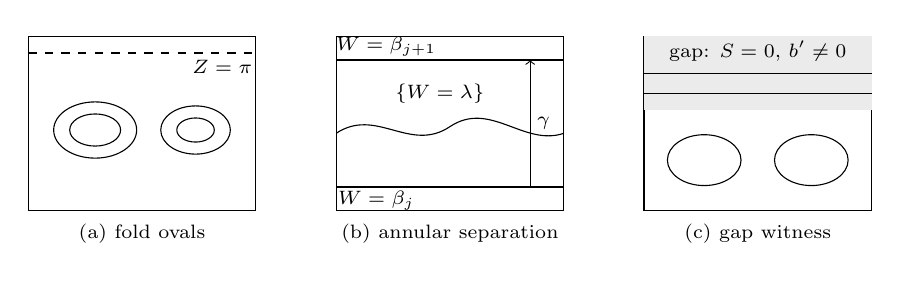
\begin{tikzpicture}[scale=0.85, every node/.style={font=\scriptsize}]
\begin{scope}
\draw (0,0) rectangle (3.4,2.6);
\node at (1.7,-0.35) {(a) fold ovals};
\draw (1.0,1.2) ellipse (0.62 and 0.42);
\draw (1.0,1.2) ellipse (0.38 and 0.24);
\draw (2.5,1.2) ellipse (0.52 and 0.36);
\draw (2.5,1.2) ellipse (0.28 and 0.18);
\draw[dashed] (0,2.35) -- (3.4,2.35);
\node at (2.9,2.15) {$Z=\pi$};
\end{scope}
\begin{scope}[xshift=4.6cm]
\draw (0,0) rectangle (3.4,2.6);
\node at (1.7,-0.35) {(b) annular separation};
\draw[thick] (0,0.35) -- (3.4,0.35);
\draw[thick] (0,2.25) -- (3.4,2.25);
\node at (0.6,0.15) {$W=\beta_j$};
\node at (0.75,2.45) {$W=\beta_{j+1}$};
\draw (0,1.15) .. controls (0.6,1.55) and (1.1,0.85) .. (1.7,1.25)
      .. controls (2.3,1.65) and (2.8,0.95) .. (3.4,1.15);
\node at (1.55,1.75) {$\{W=\lambda\}$};
\draw[->] (2.9,0.35) -- (2.9,2.25);
\node at (3.1,1.3) {$\gamma$};
\end{scope}
\begin{scope}[xshift=9.2cm]
\draw (0,0) rectangle (3.4,2.6);
\node at (1.7,-0.35) {(c) gap witness};
\fill[black!8] (0,1.5) rectangle (3.4,2.6);
\node at (1.7,2.38) {gap: $S=0$, $b'\neq0$};
\draw (0,1.75) -- (3.4,1.75);
\draw (0,2.05) -- (3.4,2.05);
\draw (0.9,0.75) ellipse (0.55 and 0.38);
\draw (2.5,0.75) ellipse (0.55 and 0.38);
\end{scope}
\end{tikzpicture}
\caption{Level-set portraits, each drawn on the fundamental square of
$\T^2$ with opposite sides identified (top/bottom are $Z=0,2\pi$;
left/right are $\xi=0,2\pi$). (a)~Regular levels of the counterexample
of Proposition~\ref{prop:counterexample}: contractible fold ovals; the
seam $\{Z=\pi\}$ is entirely critical. (b)~The annulus between
consecutive zeros of $\sqrt S$: when the boundary plateaus differ, a
Sard-regular intermediate level separates the ends and some component is
freely homotopic to a horizontal circle
(Lemmas~\ref{lem:annulus-top} and~\ref{lem:annular}); $\gamma$ is the
transverse arc of the mod-$2$ pairing. (c)~The compensated-gap witness
of Proposition~\ref{prop:gapwitness}: horizontal regular levels inside
the gap are freely homotopic to a horizontal circle.}
\label{fig:portraits}
\end{figure}

\begin{theorem}[Full single-mode strata]\label{thm:full}
Let $W$ be any member of the class \eqref{eq:full-class} satisfying
Hypotheses~\ref{hyp:v} and~\ref{hyp:conf}. Then
\[
  \lim_{T\to\infty}\oint S(Z)\,\bar V_T(Z)\,dZ=0;
\]
in particular the backward Ces\`aro mean $\Fbar$ exists and equals $0$.
\end{theorem}

\begin{proof}
By Lemma~\ref{lem:flux},
$\frac1T\int_{-T}^0\Phi\,d\tau=\frac{k^2}{4\pi}\oint S\,\bar V_T\,dZ$,
so the displayed limit is exactly the statement that $\Fbar$ exists and
vanishes.

Let $z_1<\dots<z_N$ be the zeros of $\sqrt S$ if finitely many, with
the lifted endpoint convention $z_{N+1}:=z_1+2\pi$; for $N=1$ the
single component $I_1=(z_1,z_1+2\pi)$ of $\Omega=\{S>0\}$ has both ends
at the same circle, and \eqref{eq:arc-matching} degenerates to the
periodicity identity $\oint b_Z\,dZ=0$ (the separation statement of
Lemma~\ref{lem:annular} is vacuous there). If the zero set is infinite
the argument below runs on the (at most countably many) connected
components $I_j$ of $\Omega$, with $S\to0$ at both ends of each
component, which is all that is used. By Lemma~\ref{lem:annular},
\eqref{eq:arc-matching} holds for every component and \emph{every}
$\tau$; averaging over $\tau\in[-T,0]$ gives, for every component,
\begin{equation}\label{eq:arc-avg}
  \int_{I_j}\bar V_T(Z)\,dZ=0 .
\end{equation}

Fix a component $I_j$ and $\eta\in(0,|I_j|/2)$. Let
$\text{collar}_\eta$ denote the two subintervals of $I_j$ within
distance $\eta$ of its ends, let
$K_\eta:=\{Z \in I_j : \operatorname{dist}(Z,\partial I_j)\ge\eta\}$ be
the complementary compact subarc, and let
$a_\eta:=\min_{K_\eta}\sqrt S>0$. By Lemma~\ref{lem:anchor} (and
$k\ge1$), on $K_\eta$,
\[
  |\partial_Z\bar V_T|\le\frac{K_0}{T\,a_\eta}
  \qquad\Longrightarrow\qquad
  \osc_{K_\eta}\bar V_T\le\frac{K_0\,|I_j|}{T\,a_\eta}
  \;\xrightarrow[T\to\infty]{}\;0 ,
\]
where $\osc_{K}f:=\sup_{K}f-\inf_{K}f$. Writing $m_T$ for the mean of
$\bar V_T$ over $K_\eta$, the zero-integral \eqref{eq:arc-avg} and the
uniform bound $|\bar V_T|\le C_v$ (Lemma~\ref{lem:vmean}) give
\[
  |m_T|\,|K_\eta|=\Bigl|\int_{K_\eta}\bar V_T\Bigr|
  =\Bigl|\int_{\text{collar}_\eta}\bar V_T\Bigr|\le 2\eta C_v ,
\]
so $\sup_{K_\eta}|\bar V_T|\le \frac{2\eta C_v}{|I_j|-2\eta}
+\osc_{K_\eta}\bar V_T$, and with $\|S\|_\infty:=\sup_\T S$,
\[
  \Bigl|\int_{I_j}S\,\bar V_T\Bigr|
  \le\|S\|_\infty\,|I_j|\Bigl(\frac{2\eta C_v}{|I_j|-2\eta}
  +\osc_{K_\eta}\bar V_T\Bigr)
  +\|S\|_\infty\cdot2\eta\,C_v .
\]
Hence for every admissible $\eta$,
\[
  \limsup_{T\to\infty}\Bigl|\int_{I_j}S\,\bar V_T\Bigr|
  \le\|S\|_\infty\Bigl(\frac{2\eta C_v\,|I_j|}{|I_j|-2\eta}
  +2\eta C_v\Bigr),
\]
and letting $\eta\to0$ shows $\int_{I_j}S\,\bar V_T\to0$ for every
component; outside $\Omega$ the integrand vanishes identically ($S=0$).
Finally,
\[
  \Bigl|\int_{I_j}S\,\bar V_T\Bigr|\le C_v\,\|S\|_\infty\,|I_j|,
  \qquad \sum_j|I_j|\le2\pi ,
\]
so dominated convergence for the series over components yields
$\oint S\,\bar V_T\,dZ\to0$.
\end{proof}

\begin{proof}[Proof of Theorem~\textup{\ref{thm:main-intro}}]
By Lemma~\ref{lem:class-cartesian}, every single-mode solution of
harmonic $k$ is a member of \eqref{eq:full-class}, so
Theorem~\ref{thm:full} applies verbatim; time-independent mean profiles
are the special case $b_\tau\equiv0$, in which
Theorem~\ref{thm:static} sharpens the conclusion to $b'\equiv0$.
\end{proof}

\begin{remark}[Gap-free case]\label{rem:gapfree}
If $\sqrt S$ has no zeros, \eqref{eq:arc-avg} is replaced by the
periodicity identity $\oint\bar V_T\,dZ=0$, and the argument runs with
$K_\eta=\T$, $a=\min\sqrt S>0$: the anchored cap gives
$\osc_\T\bar V_T\to0$, the zero integral forces the near-constant to
$0$, and $\oint S\,\bar V_T\to0$ directly.
\end{remark}

\begin{remark}[A saturating candidate at simple zeros]
\label{rem:saturating}
The backward-sharpening front candidate concentrated shear growth at a
simple zero $z_j$ of $\sqrt S$, exactly saturating
Lemma~\ref{lem:anchor} (which alone therefore cannot exclude it), and
its zero circles are arranged to be critical ($|b_Z|\le|X_0'|$ there), hence exempt from
Hypothesis~\ref{hyp:conf}. It is excluded by Lemma~\ref{lem:annular}:
the exemption protects the zero circles only, while the separating
levels at values strictly between the boundary plateaus are regular and
wind. Hypothesis~\ref{hyp:conf} acts here through \emph{global
separation}, not through local winding at the front.
\end{remark}

\begin{remark}[One separation device, two analytic drivers]
\label{rem:unified}
The horizontal-level separation argument appears three times in
this paper: in the spectral gaps (Step~3 of Theorem~\ref{thm:static} is
the degenerate case where a boundary plateau thickens to an interval),
on the arcs between consecutive zeros (Lemma~\ref{lem:annular}), and on
the cylinder ends (Theorem~\ref{thm:cylinder}). The whole theorem can
be organized around Lemma~\ref{lem:annulus-top}; what differs between
the two regimes is the analytic driver that the separation feeds ---
the secular growth of Step~1 for time-independent mean profiles, the
anchored cap of Lemma~\ref{lem:anchor} in general.
\end{remark}

\begin{remark}[Conserved quantities; Ces\`aro-only convergence]
\label{rem:consistency}
On the class \eqref{eq:full-class}, $\mean{u^3}\equiv0$ and the squared
modal amplitude $S$ is pointwise conserved (Lemma~\ref{lem:class-cartesian}).
Theorem~\ref{thm:full} proves that the backward Ces\`aro mean of the
flux exists and equals zero; no pointwise limit of $\Phi(\tau)$ as
$\tau\to-\infty$ is asserted, and none holds in general. A rigorous
oscillatory example (a $k=1$ member of the polar sector
\eqref{eq:polar-form}): take
\[
  A=1+\cos Z,\qquad \varphi_0=0,\qquad
  b=\delta\,(1+\cos Z)\sin Z\,\sin\tau,\qquad
  0<|\delta|\le\tfrac12 ,
\]
so that $B=\delta(1+\cos Z)\sin Z\,(1-\cos\tau)$. Both velocities are
bounded uniformly in $\tau$; every snapshot is a shear (a
$Z$-dependent $\xi$-shift, isotopic to the identity) of the
Proposition~\ref{prop:counterexample} portrait with parameter
$\varepsilon=\delta\sin\tau$, $|\varepsilon|\le\tfrac12$, hence
satisfies Hypothesis~\ref{hyp:conf}; and by Lemma~\ref{lem:flux},
$\Phi(\tau)=\tfrac{5\delta}{8}\sin\tau$: oscillatory, with zero
Ces\`aro mean.
\end{remark}

\section{The cylinder}\label{sec:cylinder}

\begin{theorem}[Cylinder version; time-independent mean profile]
\label{thm:cylinder}
Let
\[
  W=b(Z)+P_0(Z)\cos\bigl(k\xi+k\,b'(Z)\tau\bigr)
   +Q_0(Z)\sin\bigl(k\xi+k\,b'(Z)\tau\bigr)
\]
on $\T_\xi\times\R_Z$, with $b,P_0,Q_0$ smooth and $S=P_0^2+Q_0^2$
bounded (in the KNSS-symmetric setting of Corollary~\ref{cor:knss},
boundedness of $S$ is supplied by the $u$-bound via
$\sup_\xi|u|=k\sqrt S$, and boundedness of $b'$ by the $v$-bound via
$\mean{v}_\xi=-b'$). If
$C_v=\sup_{\tau\le0}\|v(\cdot,\cdot,\tau)\|_{L^\infty}<\infty$ and,
for a.e.\ $\tau\le0$ --- equivalently, by the shear conjugacy of
Lemma~\ref{lem:class-static}, for one $\tau$ --- no regular level
component of $W(\cdot,\cdot,\tau)$ is freely homotopic to a horizontal
circle $\{Z=\mathrm{const}\}$ (equivalently, generates
$H_1(\T_\xi\times\R;\mathbb Z)$), then $b'\equiv0$: the mean profile is
constant. In particular the pointwise flux density vanishes,
$\mean{W_Zu^2}_\xi=\tfrac{k^2}2\,b'S\equiv0$, and with it every average
of it.
\end{theorem}

\begin{proof}
Steps 1--2 of Theorem~\ref{thm:static} are local and apply verbatim:
$b''\equiv0$ on $\Omega=\{S>0\}$. Step 3 applies verbatim on any
bounded gap; on an unbounded gap $I$ the same argument works: the
horizontal line $\{Z=Z^*\}$, $Z^*\in I$ with $b'(Z^*)\neq0$, chosen at
a Sard-regular value as before, is a regular level component (regular
since $|\nabla W|=|b'(Z^*)|\neq0$; a \emph{complete} component because,
$b$ being strictly monotone on a collar $U\ni Z^*$ where $b(Z)=c^*$ only
at $Z=Z^*$, the circle $\{Z=Z^*\}$ is open in the level $\{W=c^*\}$ and,
being compact, closed in it) which is a circle in
$\T_\xi\times\R$ freely homotopic to $\{Z=\mathrm{const}\}$, generating
$H_1(\T_\xi\times\R;\mathbb Z)$.
The density argument of Step 4 then gives $b''\equiv0$ on $\R$, so
$b'\equiv c_0$. It remains to exclude $c_0\neq0$ without periodicity:
if $c_0\neq0$ then, with $S$ bounded, $W=c_0Z+O(1)$, so every regular
value $\lambda$ of sufficiently large absolute value has nonempty
compact level set $\{W=\lambda\}$ contained in a slab and separating
the two ends of $\T_\xi\times\R$ ($W-\lambda$ has opposite signs near
the two ends, since $W=c_0Z+O(1)$ with $c_0\neq0$).
Lemma~\ref{lem:annulus-top}, applied on a slab containing this level,
produces a component freely homotopic to a horizontal circle, violating
the hypothesis. Hence $c_0=0$, i.e.\ $b'\equiv0$; the flux statement follows from
Lemma~\ref{lem:flux}.
\end{proof}

\begin{remark}\label{rem:cylinder-full}
We do not claim the time-dependent theorem on the cylinder. The
per-arc machinery of Section~\ref{sec:full} is local and applies to
bounded components of $\{S>0\}$, but the behavior at unbounded
components requires additional end hypotheses (integrability of the
weight and a far-field normalization of the averaged shear), and we
leave the formulation and proof of an optimal cylinder statement for
time-dependent mean profiles open.
\end{remark}

\section{Sharpness of the hypotheses}\label{sec:sharpness}

\begin{proposition}[Dropping the $v$-bound]\label{prop:counterexample}
Let $0<|\varepsilon|\le\tfrac12$ and let
\[
  W_\varepsilon(\xi,Z,\tau)
  =b_\varepsilon(Z)+A(Z)\sin\bigl(\xi+b_\varepsilon'(Z)\,\tau\bigr),
  \qquad A=1+\cos Z,\quad b_\varepsilon=\varepsilon(1+\cos Z)\sin Z
\]
(the $k=1$ solution \eqref{eq:static-class} with
$(P_0,Q_0)=(0,\,1+\cos Z)$, written in the polar form of
Remark~\ref{rem:polar}; here $S=A^2$). Then $W$, $u$, $w$ are uniformly
bounded on $\tau\le0$; all regular level components are contractible
for all $\tau$, so Hypothesis~\ref{hyp:conf} holds --- indeed in the
stronger confinement form of Corollary~\ref{cor:knss}; and
\[
  \Fbar=\frac{\varepsilon}{4\pi}\oint(\cos Z+\cos2Z)(1+\cos Z)^2\,dZ
  =\frac{\varepsilon}{4\pi}\Bigl(2\pi+\frac{\pi}2\Bigr)
  =\frac{5\varepsilon}{8}\;\neq\;0 .
\]
Here $A\,b_\varepsilon''\not\equiv0$, so $v$ grows linearly in
$|\tau|$: the example satisfies every hypothesis of
Theorem~\ref{thm:static} except Hypothesis~\ref{hyp:v}, and it is
excluded exactly and only by that hypothesis.
\end{proposition}

\begin{proof}
Exactness of the solution is Lemma~\ref{lem:class-static}. For
contractibility at $\tau=0$, write the level structure explicitly: the
level $\{W_\varepsilon(\cdot,\cdot,0)=\lambda\}$ is
$\{\sin\xi=g_\lambda(Z)\}$ with
$g_\lambda:=(\lambda-b_\varepsilon)/A$ on
$\{A\neq0\}=\T\setminus\{\pi\}$. Over each connected component of
$\{|g_\lambda|<1\}$ the level consists of the two $\xi$-branches
$\arcsin g_\lambda$ and $\pi-\arcsin g_\lambda$, which join where
$|g_\lambda|=1$; a component of the level closes either as a
\emph{fold oval} (both ends of the $Z$-interval at the \emph{same}
sign of $g_\lambda=\pm1$), which is contractible, or as a curve
winding once in $\xi$ (ends at \emph{opposite} signs), which is not.
Winding in $Z$ is impossible for $\lambda\neq0$: a component winding
in $Z$ surjects onto the $Z$-circle, hence meets $\{Z=\pi\}$, where
$W_\varepsilon$ vanishes identically, so any level meeting it has
$\lambda=0$. Now the envelopes factorize:
\[
  b_\varepsilon+A=(1+\cos Z)\,(1+\varepsilon\sin Z),\qquad
  b_\varepsilon-A=-(1+\cos Z)\,(1-\varepsilon\sin Z),
\]
and for $|\varepsilon|\le\tfrac12$ both factors
$1\pm\varepsilon\sin Z$ are strictly positive, so
$b_\varepsilon+A\ge0\ge b_\varepsilon-A$ with equality only at
$Z=\pi$. Hence for $\lambda>0$ every finite end of a component of
$\{|g_\lambda|<1\}$ has $g_\lambda=+1$ (the value $g_\lambda=-1$,
i.e.\ $\lambda=b_\varepsilon-A\le0$, is impossible), and for
$\lambda<0$ symmetrically $g_\lambda=-1$: all ends carry the same
sign, so every regular level component with $\lambda\neq0$ is a fold
oval, hence contractible (the two $\xi$-branches coalesce at
$\xi=\pi/2$ where $g_\lambda=1$, resp.\ $\xi=-\pi/2$ where
$g_\lambda=-1$, and the defining $Z$-interval excludes $\pi$, so the
closed curve is an embedded oval). It remains to dispose of
$\lambda=0$: since
\[
  W_\varepsilon(\xi,Z,0)
  =(1+\cos Z)\bigl(\sin\xi+\varepsilon\sin Z\bigr),
\]
the zero level is the union of the seam $\{Z=\pi\}$ and the graphs
$\{\sin\xi=-\varepsilon\sin Z\}$; on the seam
$\nabla W_\varepsilon\equiv0$ (both terms of each partial derivative
carry the vanishing factor), and the closures of the graphs meet the
seam (at $Z=\pi$ they reach $\sin\xi=0$), so every connected component
of the zero level contains critical points: $\lambda=0$ is a critical
value and its components are not regular level components --- exempt
under either reading of Remark~\ref{rem:conventions}. (For
corroboration, the off-seam critical points of
$W_\varepsilon(\cdot,\cdot,0)$, at $\sin\xi=\pm1$, reduce under
$t=\tan(Z/2)$ to the cubics
\[
  t^3+3\varepsilon t^2+t-\varepsilon=0,\qquad
  t^3-3\varepsilon t^2+t+\varepsilon=0 ,
\]
whose derivatives $3t^2\pm6\varepsilon t+1$ have negative discriminant
$36\varepsilon^2-12\le-3$ for $|\varepsilon|\le\tfrac12$: exactly one
maximum and one minimum away from the critical circle, consistent with
the pure-oval portrait; see Figure~\ref{fig:portraits}(a). For
$|\varepsilon|$ large the positivity conclusion from the factorization
fails, opposite-sign connections appear, and regular levels wind ---
the restriction on $\varepsilon$ is what makes the example a
hypothesis-respecting witness.) Contractibility is preserved for all
$\tau$ because the evolution is the shear conjugacy $H_\tau$ of
Lemma~\ref{lem:class-static}, a diffeomorphism of $\T^2$ isotopic to
the identity. The flux integral is elementary:
$b_\varepsilon'=\varepsilon(\cos Z+\cos2Z)$ and
$\oint(\cos Z+\cos2Z)(1+\cos Z)^2\,dZ=2\pi+\tfrac\pi2$. The linear
growth of $v$ is the secular mechanism of \eqref{eq:v-static}: here
$\sqrt S\,|b_\varepsilon''|=|A\,b_\varepsilon''|\not\equiv0$, with
predicted asymptotic slope $\max_Z|A\,b_\varepsilon''|$. The
computational claims (PDE residual below $10^{-6}$ on a float64 grid,
the exact flux value, the linear $v$-growth with fitted slope matching
$\max_Z|A\,b_\varepsilon''|$) are checked by the ancillary script
\texttt{counterexample\_check.py} at $\varepsilon=0.3$
(Appendix~\ref{app:verification}); the contractibility claim is proved
analytically above, not by the script.
\end{proof}

\begin{proposition}[Admitting a horizontal level: the compensated-gap
witness]\label{prop:gapwitness}
Let $A$ be smooth, not identically zero, with
$\operatorname{supp}A\subset S_0$ for a closed interval
$S_0\subsetneq\T$, and let $V$ be a smooth periodic shear with
$V\equiv c\neq0$ on a neighborhood of $S_0$, $\oint_\T V\,dZ=0$, and
all the compensating variation of $V$ located inside the gap
$\T\setminus S_0$. Set $b(Z):=\int_0^Z V$ and let $W$ be the $k=1$
solution \eqref{eq:static-class} with this time-independent $b$ and
$(P_0,Q_0)=(0,A)$, so $S=A^2$ (polar form of Remark~\ref{rem:polar},
$\theta=\xi+b'(Z)\tau$). Then both velocity components of $W$ are
uniformly bounded (so Hypothesis~\ref{hyp:v} holds), and
\[
  \Fbar=\frac1{4\pi}\oint b'A^2\,dZ=\frac{c}{4\pi}\oint A^2\,dZ\neq0 ;
\]
the hypothesis of Theorem~\ref{thm:static} that fails is exactly
Hypothesis~\ref{hyp:conf}: horizontal regular levels inside the gap are
freely homotopic to a horizontal circle (Figure~\ref{fig:portraits}(c)).
\end{proposition}

\begin{proof}
$b$ is smooth and periodic since $\oint V=0$. On a neighborhood of
$\operatorname{supp}A$ one has $b'=V\equiv c$, hence $b''\equiv0$
there, while $A\equiv A'\equiv0$ outside $S_0$; so $A\,b''\equiv0$ on
$\T$, the secular coefficient $\sqrt S\,b''$ vanishes identically, and
$v=-b'-A'\sin\theta-A\cos\theta\,b''\tau=-b'-A'\sin\theta$ is bounded
uniformly in $\tau$, as is $u=A\cos\theta$:
Hypothesis~\ref{hyp:v} holds. The flux value is
Lemma~\ref{lem:flux} with $b'A^2=cA^2$ supported in $S_0$. Since the
flux is nonzero, Theorem~\ref{thm:static} forces a violated
hypothesis, and the only remaining candidate is
Hypothesis~\ref{hyp:conf}; explicitly, $V$ has zero mean and equals
$c\neq0$ near $S_0$, so $b'\neq0$ somewhere in the interior of the gap
$\{S=0\}$, and exactly as in Step~3 of Theorem~\ref{thm:static} a
Sard-regular value there produces a horizontal regular level component
$\{Z=Z^*\}$, freely homotopic to a horizontal circle (integer class
$(1,0)$).
\end{proof}

\begin{remark}[Hypothesis sharpness]\label{rem:table}
\emph{Drop Hypothesis~\ref{hyp:v}}:
Proposition~\ref{prop:counterexample} carries flux $5\varepsilon/8$
while satisfying Hypothesis~\ref{hyp:conf} in its strongest
(full-contractibility) form. \emph{Drop Hypothesis~\ref{hyp:conf}}:
Proposition~\ref{prop:gapwitness} carries flux
$\frac{c}{4\pi}\oint A^2\,dZ$ while satisfying
Hypothesis~\ref{hyp:v}. Thus each hypothesis of
Theorem~\ref{thm:main-intro} is individually necessary --- within every
fixed harmonic-$k$ stratum, by the covering transfer of
Remark~\ref{rem:sharpness-k} below --- and a fortiori neither
hypothesis of Corollary~\ref{cor:knss} can be dropped.
\end{remark}

\begin{remark}[Sharpness at every harmonic]\label{rem:sharpness-k}
Both witnesses are stated at $k=1$; the covering construction transfers
them to every harmonic. For a harmonic-$1$ solution $W_1$ of
\eqref{eq:static-class} set
\[
  W_k(\xi,Z,\tau):=W_1(k\xi,\,Z,\,k\tau).
\]
Then $W_k$ is the harmonic-$k$ solution \eqref{eq:static-class} with
the same $(b,X_0)$: its phase is $k\xi+k\,b'(Z)\tau$. For the two
witnesses of this section the status of each hypothesis is preserved
under the transfer: Proposition~\ref{prop:counterexample}'s levels stay
contractible (a null-homotopic component lifts to null-homotopic
components), and Proposition~\ref{prop:gapwitness}'s horizontal circle
$\{Z=\mathrm{const}\}$ is its own $\eta_k$-preimage, hence stays
horizontal. This cover-stability is a feature of stating
Hypothesis~\ref{hyp:conf} by free homotopy: the integer class $\pm(1,0)$
is neither created nor destroyed by the cover, whereas its mod-$2$
reduction is unstable --- $\cos(\xi-Z)$ has class $(1,1)$ and its $k=2$
cover $\cos(2\xi-Z)$ has class $(1,2)$, both admissible here, yet
$(1,2)\equiv(1,0)$ mod~$2$ would be spuriously forbidden by a mod-$2$
condition. First,
$v_k(\xi,Z,\tau)=v_1(k\xi,Z,k\tau)$, so $\sup|v|$ is unchanged (and
$u_k=k\,u_1(k\xi,\cdot,k\tau)$ stays bounded). Second, at each time
$\tau$ the level sets of $W_k(\cdot,\cdot,\tau)$ are the preimages of
the level sets of $W_1(\cdot,\cdot,k\tau)$ under the $k$-fold cover
$\eta_k(\xi,Z)=(k\xi,Z)$ of $\T^2$, with the same critical values
(since $\nabla W_k=(k\,\partial_\xi W_1,\partial_ZW_1)\circ\eta_k$): a
null-homotopic regular component lifts to $k$ disjoint null-homotopic
circles (a null-homotopic loop lifts to loops in any finite cover),
while a horizontal circle $\{Z=Z^*\}$ is its own preimage. By
Lemma~\ref{lem:flux} (same $b$ and $S$, harmonic $k$) the flux gains
exactly the factor $k^2$. Applied to
Proposition~\ref{prop:counterexample} this produces, for every $k$, the
witness
$W_{\varepsilon,k}=b_\varepsilon+A\sin\bigl(k\xi+k\,b_\varepsilon'\tau\bigr)$
with $\Fbar=5k^2\varepsilon/8$ and all regular level components still
contractible; applied to Proposition~\ref{prop:gapwitness}, a witness
with $\Fbar=\frac{k^2c}{4\pi}\oint A^2\,dZ$, bounded velocities, and a
horizontal regular level component. Hence the sharpness statements of
Remark~\ref{rem:table} hold within every fixed harmonic-$k$ stratum,
not merely for the union over $k$.
\end{remark}

\section{Open problems and scope}\label{sec:open}

\begin{openproblem}[Multi-mode flux rigidity]\label{op:multimode}
Does the backward Ces\`aro limit \eqref{eq:fmean} exist and equal zero
for every ancient solution of \eqref{eq:pde} on $\T^2$ satisfying
Hypotheses~\ref{hyp:v} and~\ref{hyp:conf}, without the single-mode
restriction?
\end{openproblem}

This is open to the best of the author's knowledge (note that even the
existence of the limit is part of the question: in the multi-mode class
$\Fbar$ may a priori be undefined), and the difficulty is structural
rather than technical. On the single-mode classes the flux is a pure
mean-shear channel (Lemma~\ref{lem:flux}); in general the fluctuation
channel $\mean{W'_Zu^2}$ is alive and the mean profile couples to an
infinite hierarchy of wave interactions.

We also record the scope of the present result precisely: it concerns the
single-mode strata only; the relation of the periodic-cell model to any
primitive hydrodynamic system (e.g.\ axisymmetric Navier--Stokes in a
thin-gap or long-wave regime) involves separate typing questions that
are not addressed here, and no claim at the primitive level is made.

\appendix

\section{Machine verification}\label{app:verification}

Four short standalone \texttt{Python} scripts accompany the paper as
ancillary files of the arXiv submission (directory \texttt{anc/},
together with a \texttt{Makefile}, a short \texttt{README}, a pinned
\texttt{requirements.txt}, and the checksum file \texttt{SHA256SUMS};
reference environment: Python~3.13.13, SymPy~1.14.0, NumPy~2.4.6). The
scripts are citable as ancillary files of the arXiv submission and are
also archived, with the paper, at
\href{https://doi.org/10.5281/zenodo.21492644}{\texttt{doi:10.5281/zenodo.21492644}}
(concept DOI, resolving to the latest version). None is load-bearing
for the proofs, which are complete above; they pin the computational
identities and make the counterexample independently checkable in one
command (\texttt{make verify}, run in the ancillary directory;
\texttt{make verify-mutations} for the corruption battery). Each script
asserts its checks and exits with nonzero status on any failure. The
counterexample of Proposition~\ref{prop:counterexample} is proved
analytically above; the grid check is an auxiliary diagnostic, and its
one expensive loop (the secular-slope grid) accepts a
\texttt{--fast} flag with the same acceptance gates (see the ancillary
\texttt{README} for timings and reference values).

\begin{itemize}
\item \texttt{cas\_class\_exactness.py} --- exact symbolic verification
of Lemmas~\ref{lem:class-cartesian} and~\ref{lem:flux}: the equivalence
of the PDE residual with the rotation law \eqref{eq:rotationlaw} (both
directions; symbolic in $k$), the exactness of the rotated solution
\eqref{eq:full-class}, conservation of $S$, the velocity formula, the
flux formula \eqref{eq:fluxformula} and the parity identity
$\mean{u^3}_\xi\equiv0$ (at $k=1,2,3$), and the compatibility of the
Cartesian and polar forms (Remark~\ref{rem:polar}): all exact CAS
zeros.
\item \texttt{counterexample\_check.py} --- float64 grid check of
Proposition~\ref{prop:counterexample} at $\varepsilon=0.3$ with no
hand-coded derivatives (space derivatives by FFT collocation from
sampled fields, time derivative by centered differences, predicted
secular slope by SymPy differentiation). Reference run: calibration
control ($b'\equiv0$) passes its acceptance gate $|\Fbar|<10^{-13}$
(the reference environment gives $7.8\times10^{-21}$; the exact value
is platform-dependent float noise); sampled-field PDE residual
$1.5\times10^{-7}$; time-mean flux $=5\varepsilon/8$ to relative error
$1.5\times10^{-16}$; fitted growth slope of $\sup|v|$ matching the
predicted $1.390564$ to relative error $2\times10^{-5}$.
\item \texttt{verify\_flux\_formula.py} --- independent symbolic checks
of the flux formula in polar and Fourier form, the parity
cancellation, and the exact counterexample integral
$\oint(\cos Z+\cos2Z)(1+\cos Z)^2\,dZ=5\pi/2$.
\item \texttt{mutation\_tests.py} --- the reproducible corruption
battery: nine single-site mathematical corruptions of the checkers ---
including a drift of the parameter $\varepsilon$ itself, caught by the
gates anchored to literal reference constants, and a corruption of the
calibration control itself --- are applied to temporary copies, and
each corrupted checker is asserted to exit nonzero.
\end{itemize}

Verification summary (reference run):

\begin{center}\footnotesize\setlength{\tabcolsep}{3pt}
\begin{tabular}{@{}llll@{}}
script & method & parameters & result (acceptance gate)\\
\hline
\texttt{cas\_class\_exactness} & symbolic & $k$ symbolic / $k\le3$ & all residuals $=0$ (exact zero)\\
\texttt{verify\_flux\_formula} & symbolic & --- & all identities exact (exact equality)\\
\texttt{counterexample\_check} & float64, FFT & $256^2$; slope $256\times4096$; & residual $1.5\times10^{-7}$ ($<10^{-6}$);\\
 & collocation, & $\tau$-step $2\times10^{-4}$; & flux rel.\ $1.5\times10^{-16}$ ($<10^{-10}$, sprd $<10^{-12}$);\\
 & $\varepsilon=0.3$ only & fit $[200,400]$ & slope rel.\ $2\times10^{-5}$ ($<10^{-2}$); cal.\ $<10^{-13}$\\
\end{tabular}\end{center}

\begin{thebibliography}{99}

\bibitem{BMTOnsager2023}
D.~W.~Boutros, S.~Markfelder, E.~S.~Titi,
\emph{On energy conservation for the hydrostatic Euler equations: an
Onsager conjecture}, Calc.\ Var.\ Partial Differential Equations
\textbf{62} (2023), no.~8, Paper No.~219.

\bibitem{BMT2024}
D.~W.~Boutros, S.~Markfelder, E.~S.~Titi,
\emph{Nonuniqueness of generalised weak solutions to the primitive and
Prandtl equations}, J.~Nonlinear Sci.\ \textbf{34} (2024), no.~4,
Paper No.~68.

\bibitem{Brenier1999}
Y.~Brenier,
\emph{Homogeneous hydrostatic flows with convex velocity profiles},
Nonlinearity \textbf{12} (1999), no.~3, 495--512.

\bibitem{CINT2015}
C.~Cao, S.~Ibrahim, K.~Nakanishi, E.~S.~Titi,
\emph{Finite-time blowup for the inviscid primitive equations of
oceanic and atmospheric dynamics}, Comm.\ Math.\ Phys.\ \textbf{337}
(2015), no.~2, 473--482.

\bibitem{Grenier1999}
E.~Grenier,
\emph{On the derivation of homogeneous hydrostatic equations},
M2AN Math.\ Model.\ Numer.\ Anal.\ \textbf{33} (1999), no.~5,
965--970.

\bibitem{HamelNadirashvili2019}
F.~Hamel, N.~Nadirashvili,
\emph{A Liouville theorem for the Euler equations in the plane},
Arch.\ Ration.\ Mech.\ Anal.\ \textbf{233} (2019), no.~2, 599--642.

\bibitem{HKN2016}
D.~Han-Kwan, T.~T.~Nguyen,
\emph{Ill-posedness of the hydrostatic Euler and singular Vlasov
equations}, Arch.\ Ration.\ Mech.\ Anal.\ \textbf{221} (2016), no.~3,
1317--1344.

\bibitem{KNSS2009}
G.~Koch, N.~Nadirashvili, G.~Seregin, V.~\v Sver\'ak,
\emph{Liouville theorems for the Navier--Stokes equations and
applications}, Acta Math.\ \textbf{203} (2009), no.~1, 83--105.

\bibitem{KMVW2014}
I.~Kukavica, N.~Masmoudi, V.~Vicol, T.~K.~Wong,
\emph{On the local well-posedness of the Prandtl and hydrostatic Euler
equations with multiple monotonicity regions},
SIAM J.~Math.\ Anal.\ \textbf{46} (2014), no.~6, 3865--3890.

\bibitem{KTVZ2011}
I.~Kukavica, R.~Temam, V.~Vicol, M.~Ziane,
\emph{Local existence and uniqueness for the hydrostatic Euler
equations on a bounded domain}, J.~Differential Equations \textbf{250}
(2011), no.~3, 1719--1746.

\bibitem{LeiZhang2011}
Z.~Lei, Q.~Zhang,
\emph{A Liouville theorem for the axially-symmetric Navier--Stokes
equations}, J.~Funct.\ Anal.\ \textbf{261} (2011), no.~8, 2323--2345.

\bibitem{LWX2024}
W.~S.~Leung, T.~K.~Wong, C.~Xie,
\emph{On the characterization, existence and uniqueness of steady
solutions to the hydrostatic Euler equations in a nozzle},
Arch.\ Ration.\ Mech.\ Anal.\ \textbf{248} (2024), no.~6,
Paper No.~116.

\bibitem{Martin2023}
C.~I.~Martin,
\emph{Liouville-type results for time-dependent stratified water flows
over variable bottom in the $\beta$-plane approximation},
Phys.\ Fluids \textbf{35} (2023), no.~10, Paper No.~106601.

\bibitem{MasmoudiWong2012}
N.~Masmoudi, T.~K.~Wong,
\emph{On the $H^s$ theory of hydrostatic Euler equations},
Arch.\ Ration.\ Mech.\ Anal.\ \textbf{204} (2012), no.~1, 231--271.

\bibitem{PeraltaSlobodeanu2023}
D.~Peralta-Salas, R.~Slobodeanu,
\emph{A Liouville-type theorem for the 3D primitive equations},
Phys.\ D \textbf{453} (2023), Paper No.~133821.

\bibitem{Renardy2009}
M.~Renardy,
\emph{Ill-posedness of the hydrostatic Euler and Navier--Stokes
equations}, Arch.\ Ration.\ Mech.\ Anal.\ \textbf{194} (2009), no.~3,
877--886.

\bibitem{Wong2015}
T.~K.~Wong,
\emph{Blowup of solutions of the hydrostatic Euler equations},
Proc.\ Amer.\ Math.\ Soc.\ \textbf{143} (2015), no.~3, 1119--1125.

\end{thebibliography}

\end{document}
